\documentclass[12pt]{article}%
\usepackage[a4paper, top=2.5cm, bottom=2.5cm, left=2.2cm, right=2.2cm]
{geometry}
\usepackage{float}
\usepackage{graphicx}
\restylefloat{table}

%---------------------------------------------------------------------------
\begin{document}
\title{Switcher}
\author{Ashley J. Robinson}
\date{\today}
\maketitle
%---------------------------------------------------------------------------
\section{Introduction}


\section{Hardware}


\section{Software}

\subsection{Peripherals}

\subsubsection{Analogue to Digital Convertors (ADCs)}

A single ADC is multiplexed to measure three voltages on the board. 

\subsubsection{Universal Asyncronhouse/Syncronhous Transceiver (UART)}

The UART is configure to run at 115200 baud with no control flow with a ring buffer interface. Trasmission from the microcontroller happens through \textbf{uartLoadOut} which adds to the \textbf{8 byte} buffer and is then unloaded from a timer. The input is not interrupt driven and is handled in the main control loop using a \textbf{5 byte} buffer that is enough to contain the longest command.

\subsubsection{Programmable Counter Array (PCA)}

The Pulse Width Modulation (PWM) is controlled from the counter array. The output runs at approximatly 96KHz with 8 bits to control the duty cycle. A high resolution for control would be favourable for this application but the frequency achieved in 16-bit mode is far too low for this application.

\subsubsection{Timers}

\textbf{Timer 0} is used as baud rate generagtion for the UART. \textbf{Timer 2} is used to trigger an Interrupt Service Routine (ISR) which runs at 4KHz. The ISR control the UART transmission, sampling of the ADC, running the controller and finally setting the PWM.

\subsection{Operation}

\begin{figure}[H]
	\centering
  	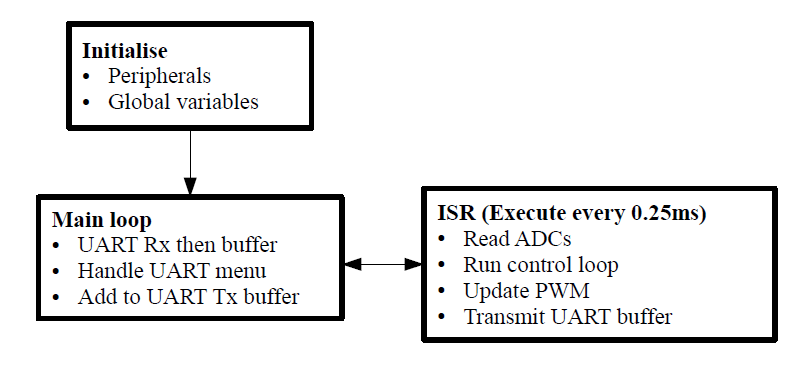
\includegraphics[width=12cm]{code.png}
  	\caption{Software overview.}
  	\label{fig:overview}
\end{figure}



\subsection{UART Menu}
\begin{table}[H]
   \centering
   \caption{UART menu}
   \label{tab:menu}
   \begin{tabular}{|p{4cm}|p{1.2cm}|p{1.8cm}|p{1.8cm}|p{4cm}|}
   \hline
      \textbf{Command}              & \textbf{Char}   &  \textbf{Send numbers}   &  \textbf{Return numbers}  &  \textbf{Notes}\\ \hline
      Enable                        & g               &  0                       &  0                        &  0                        \\ \hline
      Disable                       & s               &  0                       &  0                        &  0                        \\ \hline
      Read ADC1                     & x               &  0                       &  4                        &  Result in mV                         \\ \hline
      Read ADC2                     & y               &  0                       &  4                        &  Result in mV                         \\ \hline
      Read ADC3                     & z               &  0                       &  4                        &  Result in mV                         \\ \hline
      Read output current           & j               &  0                       &  4                        &  Result in mA              \\ \hline
      Set output voltage            & v               &  4                       &  0                        &  Send value in mV         \\ \hline
      Set otuput current            & c               &  4                       &  0                        &  Send value in mA    \\ \hline
      Set controller P              & p               &  4                       &  0                        &  Value is divide by 10    \\ \hline
      Set controller I              & i               &  4                       &  0                        &  Value is divide by 10         \\ \hline
      Set input voltage upper limit & u               &  4                       &  0                        &  Send value in mV             \\ \hline
      Set input voltage lower limit & l               &  4                       &  0                        &  Send value in mV         \\ \hline
   \end{tabular}
\end{table}

       
%---------------------------------------------------------------------------
\end{document}
